\documentclass[11pt]{article}
\usepackage[a4paper,margin=1in]{geometry}
\usepackage[T1]{fontenc}
\usepackage[utf8]{inputenc}
\usepackage{lmodern}
\usepackage{microtype}
\usepackage{amsmath,amssymb}
\usepackage{booktabs}
\usepackage{array}
\usepackage{graphicx}
\usepackage{xcolor}
\usepackage{placeins}
\usepackage{tikz}
\usetikzlibrary{positioning,arrows.meta,fit}
\usepackage[numbers,sort&compress]{natbib}
\usepackage[colorlinks=true,linkcolor=blue!50!black,citecolor=blue!50!black,urlcolor=blue!50!black]{hyperref}
\usepackage[capitalise,nameinlink]{cleveref}

\newcommand{\PFtgtA}{17.0}
\newcommand{\PFrichA}{81.9}
\newcommand{\PFabsA}{78.4}
\newcommand{\PFtgtB}{37.2}
\newcommand{\PFrichB}{80.2}
\newcommand{\PFabsB}{61.8}
\newcommand{\PFtgtC}{54.7}
\newcommand{\PFrichC}{79.9}
\newcommand{\PFabsC}{44.8}
\newcommand{\PFtgtD}{70.4}
\newcommand{\PFrichD}{79.4}
\newcommand{\PFabsD}{28.5}
\newcommand{\PFuniA}{24.9}
\newcommand{\PFuniB}{39.1}
\newcommand{\PFuniC}{60.2}
\newcommand{\PFuniD}{69.9}
\newcommand{\CFtgtA}{13.9}
\newcommand{\CFrichA}{81.4}
\newcommand{\CFabsA}{83.6}
\newcommand{\CFtgtB}{39.4}
\newcommand{\CFrichB}{81.8}
\newcommand{\CFabsB}{59.6}
\newcommand{\CFtgtC}{60.5}
\newcommand{\CFrichC}{80.8}
\newcommand{\CFabsC}{39.0}
\newcommand{\CFtgtD}{71.8}
\newcommand{\CFrichD}{80.4}
\newcommand{\CFabsD}{27.0}
\newcommand{\CFuniA}{24.4}
\newcommand{\CFuniB}{38.2}
\newcommand{\CFuniC}{60.5}
\newcommand{\CFuniD}{73.4}
\newcommand{\MPtgtA}{6.2}
\newcommand{\MPrichA}{68.8}
\newcommand{\MPabsA}{91.4}
\newcommand{\MPtgtB}{23.5}
\newcommand{\MPrichB}{67.6}
\newcommand{\MPabsB}{72.9}
\newcommand{\MPtgtC}{44.7}
\newcommand{\MPrichC}{66.9}
\newcommand{\MPabsC}{51.2}
\newcommand{\MPtgtD}{52.8}
\newcommand{\MPrichD}{65.9}
\newcommand{\MPabsD}{44.0}
\newcommand{\MPuniA}{18.3}
\newcommand{\MPuniB}{32.1}
\newcommand{\MPuniC}{47.1}
\newcommand{\MPuniD}{59.5}
\newcommand{\HWtgtA}{1.0}
\newcommand{\HWrichA}{47.4}
\newcommand{\HWabsA}{98.4}
\newcommand{\HWtgtB}{11.4}
\newcommand{\HWrichB}{48.8}
\newcommand{\HWabsB}{88.0}
\newcommand{\HWtgtC}{18.7}
\newcommand{\HWrichC}{48.2}
\newcommand{\HWabsC}{78.2}
\newcommand{\HWtgtD}{32.5}
\newcommand{\HWrichD}{49.9}
\newcommand{\HWabsD}{61.9}
\newcommand{\HWuniA}{17.1}
\newcommand{\HWuniB}{24.4}
\newcommand{\HWuniC}{29.5}
\newcommand{\HWuniD}{45.7}
\newcommand{\KDFtgtA}{7.5}
\newcommand{\KDFrichA}{67.9}
\newcommand{\KDFabsA}{91.0}
\newcommand{\KDFtgtB}{22.1}
\newcommand{\KDFrichB}{66.4}
\newcommand{\KDFabsB}{73.5}
\newcommand{\KDFtgtC}{37.7}
\newcommand{\KDFrichC}{65.8}
\newcommand{\KDFabsC}{56.5}
\newcommand{\KDFtgtD}{54.1}
\newcommand{\KDFrichD}{62.6}
\newcommand{\KDFabsD}{40.4}
\newcommand{\KDFuniA}{16.4}
\newcommand{\KDFuniB}{22.6}
\newcommand{\KDFuniC}{41.7}
\newcommand{\KDFuniD}{56.9}
\newcommand{\KPFtgtA}{9.8}
\newcommand{\KPFrichA}{79.9}
\newcommand{\KPFabsA}{88.1}
\newcommand{\KPFtgtB}{36.6}
\newcommand{\KPFrichB}{77.2}
\newcommand{\KPFabsB}{61.9}
\newcommand{\KPFtgtC}{55.6}
\newcommand{\KPFrichC}{77.9}
\newcommand{\KPFabsC}{43.4}
\newcommand{\KPFtgtD}{64.2}
\newcommand{\KPFrichD}{76.6}
\newcommand{\KPFabsD}{32.3}
\newcommand{\KPFuniA}{22.2}
\newcommand{\KPFuniB}{37.4}
\newcommand{\KPFuniC}{59.6}
\newcommand{\KPFuniD}{69.0}
\newcommand{\PFCtgtA}{11.6}
\newcommand{\PFCrichA}{80.6}
\newcommand{\PFCabsA}{84.5}
\newcommand{\PFCtgtB}{39.1}
\newcommand{\PFCrichB}{81.8}
\newcommand{\PFCabsB}{59.4}
\newcommand{\PFCtgtC}{58.5}
\newcommand{\PFCrichC}{79.6}
\newcommand{\PFCabsC}{40.2}
\newcommand{\PFCtgtD}{69.7}
\newcommand{\PFCrichD}{79.0}
\newcommand{\PFCabsD}{29.4}
\newcommand{\PFCuniA}{25.0}
\newcommand{\PFCuniB}{39.7}
\newcommand{\PFCuniC}{61.0}
\newcommand{\PFCuniD}{71.0}
\newcommand{\PFdKone}{+10.8}
\newcommand{\PFdKoneLo}{+6.2}
\newcommand{\PFdKoneHi}{+15.3}
\newcommand{\NRuns}{360}

\newcommand{\K}{K}

\title{Scarce Words in a Rich Vocabulary:\\
A Controlled Study of Low-Data Isolated {Indian} Sign Language Recognition from Landmarks}
\author{Vidit Gupta\thanks{Correspondence: \texttt{viditanupgupta@gmail.com}.} \and [Co-authors]}
\date{Preprint, September 2026}

\begin{document}
\maketitle

\begin{abstract}
Most sign languages have only a few hundred labelled video clips, and even within a
well-documented language many words have just a handful of examples. We study this regime
with a controlled benchmark built on a 30-word isolated Indian Sign Language (ISL) corpus of
634 clips from 84 signers or sessions. Test sets are signer-independent, fixed per seed and
shared by every model and every data budget. Training subsets are nested, and all models
share one fixed-step training recipe without validation-based model selection. Eight
\emph{target} words receive $K\in\{1,2,4,8\}$ training clips, either alongside 22 words that
keep all their clips (\emph{scarce} protocol) or alongside 22 words that are equally limited
(\emph{uniform} protocol). We compare 14 landmark-based models across 360 training runs:
recurrent and Transformer baselines, a graph-attention network, spectral models,
Koopman/dynamic-mode-decomposition (DMD) models and ablations, and four part-factorised
Transformers. Three findings stand out. (i) A part-factorised front end (separate body, hand
and lip encoders, a shared mirrored hand encoder, presence masks and part dropout) is the
largest single gain. At the same parameter count it raises target-word accuracy over a
landmark Transformer by 11--17 points at every $K$ ($p<0.003$, paired McNemar). (ii) Scarce
words are \emph{absorbed} by rich ones. With one example, 78--98\,\% of target clips are
predicted as a rich word. Holding the target words' data fixed, giving the other words their
full data never significantly helps the target words: all 17 significant differences are
drops, of up to 16 points. (iii) Koopman/DMD features, a cosine classifier and mixup with
label smoothing give no reliable gain in this regime. We will release the protocol, code and all
per-run predictions. Four graph-convolutional baselines are withheld while an implementation
audit is completed.
\end{abstract}

% ==========================================================================================
\section{Introduction}

Isolated sign language recognition (ISLR) has advanced quickly on large corpora such as
WLASL~\citep{li2020wlasl}, INCLUDE~\citep{sridhar2020include} and the Google ASL Signs
competition~\citep{kaggle2023aslsigns}. Two facts limit how far these results carry over.
First, most of the world's sign languages have far less annotated data. Second, the
vocabulary of even a well-resourced language has a long tail, and a recogniser deployed in a
classroom or a clinic must learn words that have been recorded a few times, next to words
that have been recorded hundreds of times. Indian Sign Language is a useful testbed for both
problems: its public corpora are small, recorded under different conditions and with few
signers per word~\citep{sridhar2020include,joshi2022cislr,patra2024hwgat}.

Few-shot results in sign recognition are hard to compare. Papers differ in whether test
signers are seen in training, in how the few examples are chosen, in whether a validation
split (drawn from the same few examples) is used for early stopping, and in whether the rare
classes are evaluated alone or inside a larger vocabulary. We fix all four choices and vary
only the model and the number of training clips per word.

\paragraph{Contributions.}
\begin{itemize}
  \item A controlled low-data ISLR protocol (\cref{sec:protocol}). It uses signer-independent
  test sets that are identical across models, data budgets and protocols, nested training
  subsets, and a fixed training budget with no validation split. A \emph{scarce-in-rich}
  setting separates the accuracy on rare words from that on common ones, and measures how
  often rare words are absorbed by common ones.
  \item A comparison of 14 landmark-based models (360 runs, 3 seeds) under one recipe. It
  includes per-clip paired significance tests, which matter here because the seed-to-seed
  standard deviation of target-word accuracy is often about 10 points.
  \item Evidence that \emph{representation structure}, not classifier design or
  regularisation, dominates at $K\le 8$: part-factorised encoders help at every $K$ and in
  both protocols, while DMD/Koopman features, cosine heads, prototype classifiers and
  mixup/label smoothing do not.
  \item Evidence that the imbalance of a scarce-in-rich vocabulary harms the scarce words.
  More data for the other words never significantly helped the target words in our
  experiments, and it significantly hurt them in 17 of 32 model--budget cells.
\end{itemize}

% ==========================================================================================
\section{Related work}

\paragraph{Isolated sign recognition from pose.}
Pose-based ISLR models consume 2D/3D keypoints from an off-the-shelf estimator such as
MediaPipe~\citep{lugaresi2019mediapipe}. Common architectures include recurrent networks,
Transformers~\citep{vaswani2017attention}, and spatio-temporal graph networks derived from
ST-GCN~\citep{yan2018stgcn}, CTR-GCN~\citep{chen2021ctrgcn} and TD-GCN~\citep{liu2024tdgcn}.
Among these are the SL-GCN ensemble~\citep{jiang2021sam} and, for ISL, HWGAT, a hierarchical
windowed graph-attention network~\citep{patra2024hwgat}. OpenHands~\citep{selvaraj2022openhands}
showed that pose-based models are data-efficient and transfer across sign languages,
including INCLUDE. Strong solutions to the Google ASL Signs competition~\citep{kaggle2023aslsigns}
combined separate treatment of hands, lips and body with interleaved depthwise temporal
convolutions and Transformer blocks. Our Conv1DFormer follows that pattern.

\paragraph{Few-shot and low-shot recognition.}
Metric-based methods classify by distance to class prototypes~\citep{snell2017proto}. Cosine
(normalised) classifiers~\citep{gidaris2018dynamic,qi2018imprinted,chen2019closer} reduce
the norm bias between classes with many and few examples. Generalised low-shot
learning~\citep{hariharan2017lowshot} and long-tailed recognition~\citep{kang2020decoupling}
study the case where rare and common classes are evaluated together. There, the classifier
tends to favour common classes, and the representation and the classifier can be analysed
separately. Our scarce protocol is a small-scale instance of this setting for sign language,
and our prototype evaluation separates the representation from the linear head. Zero-shot
sign recognition from textual descriptions~\citep{bilge2019zeroshot} is complementary to
our setting.

\paragraph{Koopman and DMD features.}
Dynamic mode decomposition~\citep{schmid2010dmd} and its delay-embedded (Hankel)
variant~\citep{arbabi2017hankel} estimate a linear operator whose spectrum summarises a
trajectory's oscillations and decay. Neural Koopman Pooling~\citep{wang2023koopman} learns
class-wise Koopman operators for skeleton action recognition and reports gains in one-shot
settings. We test whether such dynamical descriptors help when only a few examples of each
sign are available.

% ==========================================================================================
\section{Data}\label{sec:data}

We use a 30-word isolated ISL corpus~\citep{gupta2026isl30}. It was assembled from four sources:
ISL500~\citep{isl500} (405 clips), INCLUDE~\citep{sridhar2020include} (164),
CISLR~\citep{joshi2022cislr} (63) and the ISLRTC dictionary~\citep{islrtc} (2). The 30 words
are those of an earlier 40-word corpus that have at least 16 clips from at least 4 distinct
signers. Two of them (\emph{brother}, \emph{me}) were topped up with additional INCLUDE
clips. The corpus has 634 clips, with 16--38 clips per word (median 17), and 84 identities.

\paragraph{Identities.}
A clip's identity is its signer when known (17 named signers), otherwise its recording
session, otherwise the clip itself. INCLUDE provides no signer labels, so we infer recording
sessions from jumps in the camera's file counter. Duplicate clips that occur in more than
one source are removed. All train/test splits are made at the identity level.

\paragraph{Vocabulary.}
The eight \emph{target} words are \emph{eat, go, hello, help, no, please, water, yes}. These are
the eight best-represented words of the earlier corpus and are kept from our previous
experiments. The 22 \emph{rich} words are \emph{brother, drink, father, food, friend, he,
market, me, mother, okay, school, she, sister, sit, student, tea, teacher, thank you, today,
what, where, you}.

\paragraph{Landmarks.}
We extract MediaPipe Holistic landmarks~\citep{lugaresi2019mediapipe} for every frame
(543 points). Leading and trailing frames without a detected hand are trimmed, and $T=30$
frames are sampled uniformly. Coordinates are centred on the mid-hip point (mid-shoulder if
the hips are not visible) and scaled by the shoulder width. We keep a reduced layout of 119
points (33 pose, $2\times21$ hand, 40 lip and 4 nose points), with missing points set to
zero. Hands are frequently undetected (in a pilot, the right hand was found in 29--65\,\% of
frames), so models that know which points are missing have an advantage.

% ==========================================================================================
\section{Protocol}\label{sec:protocol}

\paragraph{Test sets.}
For each seed, whole identities are moved to the test set, in a seeded order, until each word
has about 25\,\% of its clips in test (at least 2, at most 20, and never more than half of a
word's clips). The test set depends only on the clip table and the seed. It is therefore
identical for every model, every $K$ and both protocols, which our report script verifies by
fingerprint. With 30 words each seed has 240 test clips: 62 from target words and 178 from
rich words, from 26 test identities (seed~0).

\paragraph{Nested training subsets.}
The training pool of each word is ordered once per (seed, word), round-robin over
identities. The $K$-clip subset is the first $K$ clips of this order. Subsets are therefore
nested ($K{=}1\subset K{=}2\subset\dots$), and already at small $K$ they span several signers.

\paragraph{Protocols.}
\emph{Scarce}: the 8 target words get $K$ clips each and the 22 rich words keep their whole
training pool (8--29 clips each). This gives 307 training clips at $K{=}1$ and 363 at $K{=}8$.
\emph{Uniform}: every word gets $K$ clips ($30K$ training clips). \emph{Vocabulary}: the
scarce protocol with the vocabulary restricted to the 8 targets ($V{=}8$, which is then
uniform), the targets plus 8 rich words ($V{=}16$), or all 30 words. In all protocols the
target words' training clips for a given (seed, $K$) are the same.

\paragraph{Training recipe (all models).}
No validation split and no early stopping: with $K\le8$ a validation split would consume the
data and select on noise. Each run trains for a fixed number of steps,
$\mathrm{clamp}(E\cdot n_\text{train}/B,\,300,\,6000)$, with batch size $B{=}16$ and $E{=}80$
epochs (60 for the CWT models). For example, scarce $K{=}8$ runs take 1\,815 steps. The
optimiser is AdamW~\citep{loshchilov2019adamw} with learning rate $10^{-3}$, weight decay
0.01, 5\,\% linear warm-up and cosine decay, gradient clipping at 1.0 and mixed precision. The
landmark augmentation is computed on the GPU. It applies an in-plane rotation of
$\pm15^\circ$, scaling by $\pm15\,\%$, a small anisotropic stretch, a translation, and
coordinate noise on detected points only, followed by a non-circular temporal warp
(speed 0.8--1.2, shift $\pm15\,\%$). We never flip horizontally, because a flip swaps the
dominant hand.

\paragraph{Metrics and statistics.}
We report top-1 accuracy on the target words, on the rich words and overall. We also report
the \emph{absorption rate}: the fraction of target-word test clips predicted as a rich word.
The \emph{prototype accuracy} is the nearest-class-mean accuracy (cosine) of the
classifier's input embedding, with class means computed from the training clips. Each
configuration is run with 3 seeds, and we give the mean $\pm$ standard deviation over seeds.
Because the seeds differ in their test signers, much of that deviation is shared by all
models. We therefore compare models \emph{per clip}. Predictions are pooled over the 3 seeds
($n{=}186$ target clips, 720 clips in all) and compared with an exact two-sided McNemar
test~\citep{mcnemar1947,dietterich1998tests} and a paired bootstrap 95\,\% confidence
interval of the accuracy difference~\citep{efron1993bootstrap}.

% ==========================================================================================
\section{Models}\label{sec:models}

All models read the same normalised landmarks and differ only in the view of the landmarks
they use (\cref{tab:models}). Hyper-parameters were fixed before the sweep and are not tuned
per model or per $K$.

\paragraph{Landmark baselines.}
MP-BiLSTM (a 2-layer BiLSTM~\citep{hochreiter1997lstm}) and MP-Transformer (a 3-layer
Transformer with $d{=}128$) both take the 225-dimensional pose+hand vector (75 points $\times$
3) of each frame. MP-Transformer is our reference model for all paired tests.

\paragraph{Graph model.}
HWGAT~\citep{patra2024hwgat} is our re-implementation, run on a 27-joint upper-body and hand
skeleton. We also ran ST-GCN, CTR-GCN, TD-GCN and a graph-Fourier model (PGF-SLR). An audit
after the sweep found implementation errors in all four: the input batch normalisation of the
three GCNs normalised over the wrong axes, and PGF-SLR averaged joints within a part before
projecting them. Their results are withheld until the corrected runs finish (\cref{sec:limits}).

\paragraph{Spectral models.}
FFT-BiLSTM uses windowed FFT magnitudes and kinematic features. CWT-BiLSTM and
CWT-Transformer use continuous-wavelet band energies of the landmark trajectories.

\paragraph{Koopman models.}
KDF-Transformer adds two dynamical components to the MP-Transformer backbone. The first is a
Hankel-DMD branch~\citep{arbabi2017hankel}. The trajectories of the upper body and of each
hand are Kalman-smoothed and delay-embedded with $d{=}8$ delays, and $r{=}3$ modes are kept
per part. This gives a 39-dimensional spectral descriptor (for each mode, $\log(1{+}|\lambda|)$,
$\sin\arg\lambda$, $\cos\arg\lambda$ and the RMS amplitude, plus per-part kinetic energy) and
9 spatial mode maps. The second is a class-wise Koopman head in the spirit of Neural Koopman
Pooling~\citep{wang2023koopman}, trained with an auxiliary loss (weight 0.3). KDF models are
trained with mixup~\citep{zhang2018mixup} ($\alpha{=}0.2$) and label smoothing
0.1~\citep{szegedy2016inception}. The ablations remove the DMD branch ($-$DMD), the Koopman
head ($-$Koopman head) or both. Removing both leaves MP-Transformer trained with mixup and
label smoothing (``MP-Transformer + mixup/LS''), which isolates the effect of the
regularisers.

\paragraph{Part-factorised models (ours).}
\begin{figure}[t]
\centering
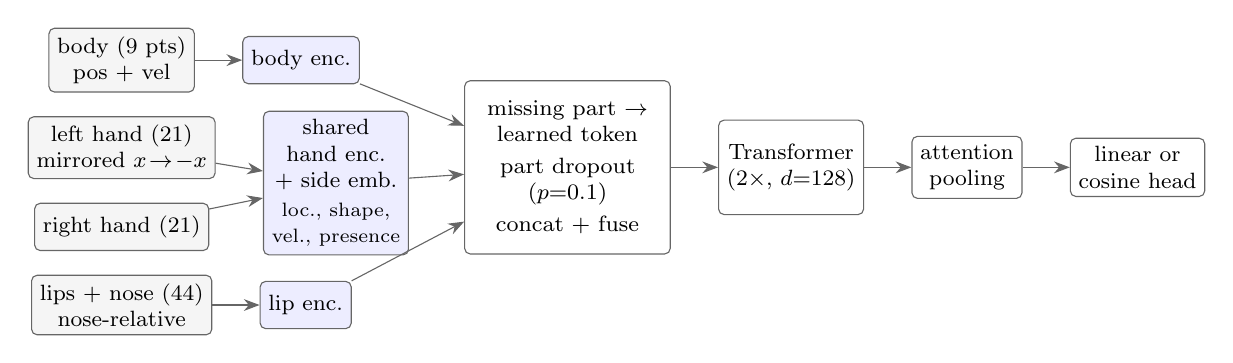
\begin{tikzpicture}[
  font=\footnotesize, node distance=3mm and 6mm,
  box/.style={draw=black!60, rounded corners=2pt, align=center, inner sep=3pt, minimum height=6mm},
  inp/.style={box, fill=black!4},
  enc/.style={box, fill=blue!7},
  arr/.style={-{Stealth[length=2mm]}, black!60}]
  \node[inp] (body) {body (9 pts)\\pos + vel};
  \node[inp, below=of body] (lh) {left hand (21)\\mirrored $x\!\to\!-x$};
  \node[inp, below=of lh] (rh) {right hand (21)};
  \node[inp, below=of rh] (face) {lips + nose (44)\\nose-relative};
  \node[enc, right=of body] (eb) {body enc.};
  \node[enc, right=of lh, yshift=-4.5mm, minimum height=16mm] (eh) {shared\\hand enc.\\+ side emb.\\[1pt]\scriptsize loc., shape,\\\scriptsize vel., presence};
  \node[enc, right=of face] (ef) {lip enc.};
  \node[box, right=7mm of eh, yshift=2mm, minimum height=22mm, text width=24mm] (mask)
       {missing part $\to$ learned token\\[2pt] part dropout ($p{=}0.1$)\\[2pt] concat + fuse};
  \node[box, right=of mask, minimum height=12mm] (tr) {Transformer\\($2\times$, $d{=}128$)};
  \node[box, right=of tr] (pool) {attention\\pooling};
  \node[box, right=of pool] (head) {linear or\\cosine head};
  \foreach \a/\b in {body/eb, lh/eh, rh/eh, face/ef} \draw[arr] (\a) -- (\b);
  \foreach \a in {eb, eh, ef} \draw[arr] (\a) -- (mask);
  \draw[arr] (mask) -- (tr); \draw[arr] (tr) -- (pool); \draw[arr] (pool) -- (head);
\end{tikzpicture}
\caption{PartFormer's front end. Each part is projected before it is normalised, so the
hand's position relative to the body is kept. Both hands share one encoder: the left hand is
mirrored and a side embedding is added. Conv1DFormer replaces the Transformer with
depthwise-temporal-convolution and Transformer blocks. KDF-PartFormer adds the DMD branch and
the Koopman head.}
\label{fig:partformer}
\end{figure}
PartFormer (\cref{fig:partformer}) encodes each frame as four part tokens:
\begin{itemize}
  \item a body token: 9 points (nose, shoulders, elbows, wrists and hips) with their
  velocities;
  \item two hand tokens from one shared encoder;
  \item a lip token: 40 lip points relative to the nose, with velocities.
\end{itemize}
A hand token combines four inputs: the hand's position in the body frame, its wrist-relative
shape normalised by size, its velocity, and a presence flag. The left hand is mirrored, so
one set of weights serves both hands and both left- and right-dominant signers, and a learned
side embedding says which hand it is. Each part is projected before layer normalisation.
Normalising the raw coordinates would erase where the hand is relative to the body, which is
part of a sign's meaning. A part that is not detected is replaced by a learned token. During
training whole parts are dropped with probability 0.1, so the model cannot rely on any one
part. The fused tokens pass through a 2-layer Transformer and attention pooling.

There are three variants:
\begin{itemize}
  \item \emph{PartFormer-cos} replaces the linear head with a cosine head (learned
  temperature, initial scale 16).
  \item \emph{Conv1DFormer} interleaves depthwise temporal convolution blocks (kernel 7) with
  Transformer blocks, following strong ASL Signs solutions.
  \item \emph{KDF-PartFormer} adds the DMD branch and the Koopman head.
\end{itemize}
All part models use mixup and label smoothing like the KDF models. The comparison with
MP-Transformer + mixup/LS therefore isolates the front end from the regularisers.

\begin{table}[t]
\centering
\small
\caption{Models. Parameters for 30 classes; training time is the mean wall-clock time of a scarce $K{=}8$ run (1\,815 steps, batch 16) on one laptop RTX~2050 GPU.}
\label{tab:models}
\begin{tabular}{lllrr}
\toprule
Model & Family & Input & Params & Train (s) \\
\midrule
MP-BiLSTM & Landmark & pose+hands (75 pts) & 2.58\,M & 100 \\
MP-Transformer & Landmark & pose+hands (75 pts) & 0.43\,M & 103 \\
\midrule
HWGAT & Graph & 27-joint skeleton & 1.21\,M & 315 \\
\midrule
FFT-BiLSTM & Spectral & FFT + kinematics & 2.95\,M & 98 \\
CWT-BiLSTM & Spectral & CWT bands & 3.28\,M & 71 \\
CWT-Transformer & Spectral & CWT bands & 0.47\,M & 72 \\
\midrule
KDF-Transformer & Koopman & pose+hands + DMD & 0.51\,M & 159 \\
KDF $-$DMD & Koopman & pose+hands (75 pts) & 0.50\,M & 140 \\
KDF $-$Koopman head & Koopman & pose+hands + DMD & 0.45\,M & 133 \\
MP-Transformer + mixup/LS & Koopman & pose+hands (75 pts) & 0.43\,M & 126 \\
\midrule
PartFormer & Part & parts (119 pts) & 0.40\,M & 158 \\
PartFormer-cos & Part & parts (119 pts) & 0.40\,M & 166 \\
Conv1DFormer & Part & parts (119 pts) & 0.60\,M & 197 \\
KDF-PartFormer & Part & parts + DMD & 0.48\,M & 193 \\
\bottomrule
\end{tabular}
\end{table}


% ==========================================================================================
\section{Results}\label{sec:results}

\subsection{Scarce words inside a 30-word vocabulary}

\begin{table}[t]
\centering
\small
\caption{Scarce protocol: top-1 accuracy (\%) on the 8 target words, which have $K$ training clips each while the other 22 words keep all their clips. Mean $\pm$ s.d.\ over 3 seeds; 62 target test clips per seed from unseen signers. Best per column in bold.}
\label{tab:scarce}
\begin{tabular}{lcccc}
\toprule
Model & $K=1$ & $K=2$ & $K=4$ & $K=8$ \\
\midrule
MP-BiLSTM & 6.1\,{\scriptsize$\pm$3.0} & 24.8\,{\scriptsize$\pm$15.1} & 38.3\,{\scriptsize$\pm$12.0} & 51.8\,{\scriptsize$\pm$15.8} \\
MP-Transformer & 6.2\,{\scriptsize$\pm$3.0} & 23.5\,{\scriptsize$\pm$7.5} & 44.7\,{\scriptsize$\pm$11.7} & 52.8\,{\scriptsize$\pm$11.7} \\
\midrule
HWGAT & 1.0\,{\scriptsize$\pm$0.9} & 11.4\,{\scriptsize$\pm$5.2} & 18.7\,{\scriptsize$\pm$2.0} & 32.5\,{\scriptsize$\pm$9.5} \\
\midrule
FFT-BiLSTM & 8.6\,{\scriptsize$\pm$3.7} & 21.7\,{\scriptsize$\pm$1.2} & 35.0\,{\scriptsize$\pm$7.3} & 46.2\,{\scriptsize$\pm$12.1} \\
CWT-BiLSTM & 11.2\,{\scriptsize$\pm$3.2} & 27.5\,{\scriptsize$\pm$11.0} & 41.4\,{\scriptsize$\pm$12.1} & 49.4\,{\scriptsize$\pm$15.4} \\
CWT-Transformer & 8.9\,{\scriptsize$\pm$4.1} & 30.0\,{\scriptsize$\pm$9.6} & 45.1\,{\scriptsize$\pm$13.7} & 62.1\,{\scriptsize$\pm$17.5} \\
\midrule
KDF-Transformer & 7.5\,{\scriptsize$\pm$1.2} & 22.1\,{\scriptsize$\pm$11.7} & 37.7\,{\scriptsize$\pm$12.7} & 54.1\,{\scriptsize$\pm$9.6} \\
\quad $-$DMD & 6.4\,{\scriptsize$\pm$1.9} & 13.0\,{\scriptsize$\pm$11.9} & 39.8\,{\scriptsize$\pm$15.7} & 54.3\,{\scriptsize$\pm$10.2} \\
\quad $-$Koopman head & 6.3\,{\scriptsize$\pm$4.8} & 18.1\,{\scriptsize$\pm$13.8} & 36.2\,{\scriptsize$\pm$16.4} & 50.2\,{\scriptsize$\pm$11.4} \\
\quad $-$both (mixup+LS only) & 4.3\,{\scriptsize$\pm$2.6} & 17.3\,{\scriptsize$\pm$10.1} & 36.6\,{\scriptsize$\pm$7.7} & 46.5\,{\scriptsize$\pm$10.6} \\
\midrule
PartFormer & \textbf{17.0\,{\scriptsize$\pm$3.5}} & 37.2\,{\scriptsize$\pm$10.2} & 54.7\,{\scriptsize$\pm$7.1} & 70.4\,{\scriptsize$\pm$10.8} \\
PartFormer-cos & 11.6\,{\scriptsize$\pm$6.3} & 39.1\,{\scriptsize$\pm$7.4} & 58.5\,{\scriptsize$\pm$4.7} & 69.7\,{\scriptsize$\pm$3.6} \\
Conv1DFormer & 13.9\,{\scriptsize$\pm$2.5} & \textbf{39.4\,{\scriptsize$\pm$14.0}} & \textbf{60.5\,{\scriptsize$\pm$7.9}} & \textbf{71.8\,{\scriptsize$\pm$11.2}} \\
KDF-PartFormer & 9.8\,{\scriptsize$\pm$3.2} & 36.6\,{\scriptsize$\pm$6.9} & 55.6\,{\scriptsize$\pm$9.5} & 64.2\,{\scriptsize$\pm$9.6} \\
\bottomrule
\end{tabular}
\end{table}


\begin{figure}[t]
\centering
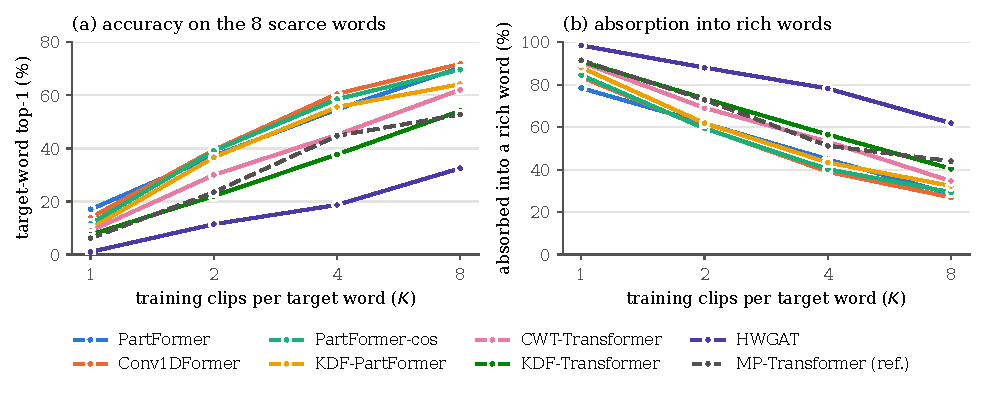
\includegraphics[width=\linewidth]{figures/scarce.pdf}
\caption{Scarce protocol, mean over 3 seeds. (a) Top-1 accuracy on the 8 target words.
(b) Share of target-word test clips predicted as one of the 22 rich words. All values, with
standard deviations, are in \cref{tab:scarce,tab:absorb}.}
\label{fig:scarce}
\end{figure}

\Cref{tab:scarce} and \cref{fig:scarce}a show target-word accuracy as $K$ grows. The four
part-factorised models form a clear top group at every $K$. With one clip per target word,
PartFormer reaches \PFtgtA\,\% against \MPtgtA\,\% for MP-Transformer. With eight clips the
best model, Conv1DFormer, reaches \CFtgtD\,\% against \MPtgtD\,\%. The landmark baselines,
the spectral models and the landmark-backbone KDF models form a second group, 15--20 points
lower. HWGAT is last at every $K$. Standard deviations over seeds are large (often around 10
points) because the three seeds hold out different signers, so we rely on per-clip paired
tests (\cref{tab:paired}).

\begin{table}[t]
\centering
\small
\caption{Paired comparison with MP-Transformer on the scarce protocol, pooled over 3 seeds (same test clips). $\Delta$: accuracy difference in points with a 95\,\% paired-bootstrap CI; $p$: exact two-sided McNemar test. Target clips: $n=186$; all clips: $n=720$.}
\label{tab:paired}
\footnotesize
\setlength{\tabcolsep}{3.5pt}
\begin{tabular}{llcccc}
\toprule
 & & \multicolumn{2}{c}{target words} & \multicolumn{2}{c}{all words} \\
\cmidrule(lr){3-4}\cmidrule(lr){5-6}
$K$ & Model & $\Delta$ [95\,\% CI] & $p$ & $\Delta$ [95\,\% CI] & $p$ \\
\midrule
1 & PartFormer & +10.8 [+6.2, +15.3] & $2.1\!\times\!10^{-5}$ & +12.3 [+9.4, +15.2] & $2.2\!\times\!10^{-15}$ \\
1 & PartFormer-cos & +6.2 [+2.3, +10.2] & 0.003 & +10.5 [+7.7, +13.4] & $1.1\!\times\!10^{-12}$ \\
1 & Conv1DFormer & +8.0 [+3.4, +12.5] & 0.001 & +11.4 [+8.5, +14.5] & $7.5\!\times\!10^{-15}$ \\
1 & KDF-PartFormer & +4.0 [+0.0, +8.5] & 0.118 & +9.2 [+6.4, +12.3] & $9.0\!\times\!10^{-10}$ \\
1 & CWT-Transformer & +2.8 [-1.1, +7.4] & 0.302 & -0.6 [-3.5, +2.5] & 0.783 \\
1 & KDF-Transformer & +1.1 [-2.3, +4.5] & 0.754 & -0.4 [-2.7, +1.9] & 0.807 \\
1 & MP-Transformer + mixup/LS & -2.3 [-5.7, +1.1] & 0.344 & -1.0 [-3.2, +1.2] & 0.435 \\
1 & HWGAT & -5.1 [-9.1, -1.7] & 0.012 & -17.2 [-20.8, -13.6] & $6.3\!\times\!10^{-20}$ \\
\midrule
2 & PartFormer & +13.1 [+6.2, +19.9] & $4.3\!\times\!10^{-4}$ & +12.7 [+9.5, +15.8] & $1.5\!\times\!10^{-14}$ \\
2 & PartFormer-cos & +15.3 [+8.0, +22.7] & $1.4\!\times\!10^{-4}$ & +14.5 [+11.1, +17.6] & $3.4\!\times\!10^{-17}$ \\
2 & Conv1DFormer & +14.8 [+7.4, +22.2] & $2.2\!\times\!10^{-4}$ & +14.3 [+11.0, +17.6] & $1.7\!\times\!10^{-16}$ \\
2 & KDF-PartFormer & +13.1 [+5.7, +20.5] & 0.001 & +10.5 [+7.5, +13.7] & $2.1\!\times\!10^{-10}$ \\
2 & CWT-Transformer & +6.2 [-0.6, +13.1] & 0.099 & +2.6 [-0.7, +5.9] & 0.145 \\
2 & KDF-Transformer & -2.3 [-8.0, +4.0] & 0.572 & -1.4 [-4.0, +1.2] & 0.314 \\
2 & MP-Transformer + mixup/LS & -6.8 [-12.5, -1.1] & 0.029 & -2.6 [-5.2, -0.1] & 0.050 \\
2 & HWGAT & -10.8 [-17.6, -4.0] & 0.003 & -16.3 [-20.2, -12.3] & $3.6\!\times\!10^{-15}$ \\
\midrule
4 & PartFormer & +11.4 [+5.1, +18.2] & 0.002 & +12.7 [+9.7, +15.9] & $2.9\!\times\!10^{-15}$ \\
4 & PartFormer-cos & +14.8 [+8.0, +21.6] & $4.2\!\times\!10^{-5}$ & +13.2 [+9.8, +16.5] & $9.1\!\times\!10^{-15}$ \\
4 & Conv1DFormer & +15.9 [+8.5, +22.7] & $4.1\!\times\!10^{-5}$ & +14.5 [+11.3, +17.6] & $2.8\!\times\!10^{-18}$ \\
4 & KDF-PartFormer & +11.9 [+5.1, +18.8] & 0.001 & +11.3 [+7.9, +14.6] & $3.2\!\times\!10^{-11}$ \\
4 & CWT-Transformer & +1.7 [-4.5, +8.0] & 0.736 & -0.3 [-3.8, +3.2] & 0.935 \\
4 & KDF-Transformer & -7.4 [-13.1, -1.7] & 0.019 & -2.6 [-5.5, +0.1] & 0.085 \\
4 & MP-Transformer + mixup/LS & -8.0 [-13.6, -2.3] & 0.013 & -3.2 [-5.8, -0.6] & 0.020 \\
4 & HWGAT & -25.0 [-33.5, -16.5] & $3.6\!\times\!10^{-8}$ & -20.1 [-24.1, -16.0] & $1.5\!\times\!10^{-20}$ \\
\midrule
8 & PartFormer & +16.5 [+10.2, +22.7] & $4.2\!\times\!10^{-7}$ & +14.5 [+11.3, +17.6] & $1.0\!\times\!10^{-17}$ \\
8 & PartFormer-cos & +15.9 [+10.2, +22.2] & $7.7\!\times\!10^{-7}$ & +14.0 [+10.8, +17.2] & $1.6\!\times\!10^{-16}$ \\
8 & Conv1DFormer & +17.0 [+10.8, +23.3] & $6.0\!\times\!10^{-7}$ & +15.3 [+12.0, +18.6] & $2.2\!\times\!10^{-19}$ \\
8 & KDF-PartFormer & +10.2 [+4.0, +16.5] & 0.002 & +10.8 [+7.7, +14.0] & $2.8\!\times\!10^{-11}$ \\
8 & CWT-Transformer & +9.1 [+3.4, +15.3] & 0.005 & +2.6 [-0.7, +5.8] & 0.151 \\
8 & KDF-Transformer & +0.0 [-5.1, +5.1] & 1.000 & -2.3 [-5.1, +0.3] & 0.113 \\
8 & MP-Transformer + mixup/LS & -6.2 [-10.8, -2.3] & 0.007 & -2.2 [-4.8, +0.4] & 0.119 \\
8 & HWGAT & -19.9 [-27.8, -11.9] & $3.3\!\times\!10^{-6}$ & -16.6 [-20.5, -12.6] & $5.5\!\times\!10^{-15}$ \\
\bottomrule
\end{tabular}
\end{table}


On the target clips, every part model is significantly better than MP-Transformer at
$K\ge2$ (gains of 10--17 points, $p\le0.002$). PartFormer is also significantly better at
$K{=}1$ (\PFdKone\ points, 95\,\% CI [\PFdKoneLo, \PFdKoneHi]). Over all 720 test clips, the
part models gain 9--15 points at every $K$ with $p<10^{-9}$. They also improve the rich
words, from about 66 to 80\,\% (\cref{tab:rich}), even though the rich words' training data
are the same in every run. The part front end is thus a better representation in general,
not only a better few-shot one. KDF-Transformer never differs significantly from its own
backbone on the target clips except at $K{=}4$, where it is worse.

\subsection{Absorption: rare words are predicted as common ones}

\Cref{fig:scarce}b and \cref{tab:absorb} show where the misclassified target clips go. At
$K{=}1$, 78\,\% (PartFormer) to 98\,\% (HWGAT) of target clips are predicted as a rich word.
In other words, nearly all errors on the rare words are confusions with common words, not
with other rare words. The rate falls steadily with $K$, to 27--32\,\% for the part models and
44\,\% for MP-Transformer at $K{=}8$. The ranking of models by absorption closely mirrors
their ranking by target accuracy.

\begin{table}[t]
\centering
\small
\caption{Effect of the rich words' data on the target words. Target-word top-1 (\%) when every word has $K$ clips (uniform) $\to$ when the 22 other words keep their full pools (scarce). The target words' training clips and all test clips are identical in the two settings. In parentheses: scarce $-$ uniform in points, pooled over 3 seeds ($n=186$ target clips); $^{*}$: exact McNemar $p<0.05$.}
\label{tab:univsscarce}
\begin{tabular}{lcccc}
\toprule
Model & $K=1$ & $K=2$ & $K=4$ & $K=8$ \\
\midrule
MP-Transformer & 11$\to$6 (-5$^{*}$) & 35$\to$23 (-11$^{*}$) & 50$\to$45 (-6) & 63$\to$53 (-10$^{*}$) \\
HWGAT & 11$\to$1 (-10$^{*}$) & 22$\to$11 (-11$^{*}$) & 26$\to$19 (-9$^{*}$) & 40$\to$33 (-7$^{*}$) \\
KDF-Transformer & 9$\to$8 (-2) & 29$\to$22 (-7) & 41$\to$38 (-4) & 57$\to$54 (-2) \\
MP-Transformer + mixup/LS & 11$\to$4 (-7$^{*}$) & 34$\to$17 (-16$^{*}$) & 48$\to$37 (-11$^{*}$) & 54$\to$47 (-7$^{*}$) \\
PartFormer & 20$\to$17 (-4) & 43$\to$37 (-6) & 66$\to$55 (-10$^{*}$) & 69$\to$70 (+2) \\
PartFormer-cos & 22$\to$12 (-10$^{*}$) & 40$\to$39 (-1) & 64$\to$59 (-5) & 71$\to$70 (+0) \\
Conv1DFormer & 20$\to$14 (-6) & 47$\to$39 (-8$^{*}$) & 61$\to$61 (-1) & 72$\to$72 (-1) \\
KDF-PartFormer & 18$\to$10 (-8$^{*}$) & 47$\to$37 (-10$^{*}$) & 65$\to$56 (-9$^{*}$) & 68$\to$64 (-3) \\
\bottomrule
\end{tabular}
\end{table}


\paragraph{Do the rich words' data help or hurt the scarce words?}
The uniform and scarce protocols give the target words exactly the same training clips and
share all test clips. The only difference is whether the 22 other words have $K$ clips or
their full pools (8--29 clips). \Cref{tab:univsscarce} compares the two. In 30 of 32
model--budget cells, target accuracy is lower in the scarce setting (one is higher, one unchanged). Seventeen of these drops
are significant (up to 16 points), and no increase is. So, in this regime, extra data for
other classes does not transfer to the scarce classes: it makes the classifier favour the
common words. The part models are the least affected. PartFormer and Conv1DFormer show no
significant loss at $K{=}8$, and PartFormer's $K{=}1$ and $K{=}2$ drops (4--6 points) are
not significant. MP-Transformer, with or without mixup/LS, and HWGAT lose 5--16 points at most budgets. The recipe does not rebalance
classes. Class-balanced sampling or logit adjustment~\citep{kang2020decoupling} is an obvious
next step that our protocol can evaluate directly.

\subsection{Effect of vocabulary size}

\begin{figure}[t]
\centering
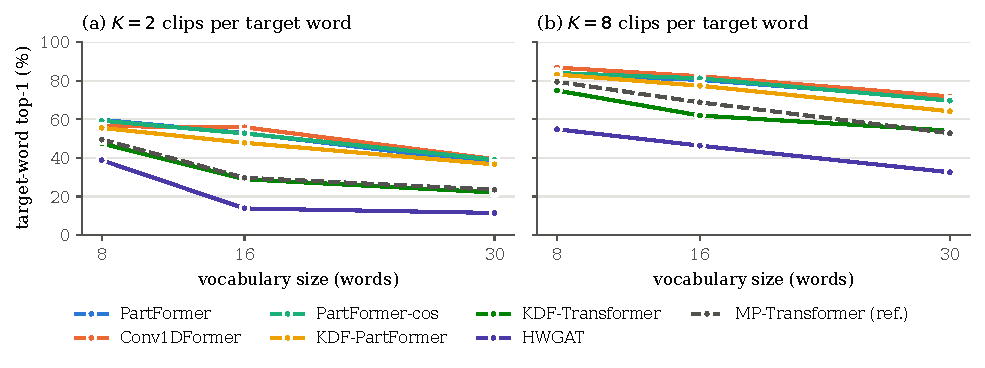
\includegraphics[width=\linewidth]{figures/vocab.pdf}
\caption{Target-word top-1 accuracy when the 8 target words are embedded in 8, 16 or 30
words (scarce protocol, mean over 3 seeds; values in \cref{tab:vocab}).}
\label{fig:vocab}
\end{figure}

\begin{table}[t]
\centering
\small
\caption{Vocabulary size: top-1 accuracy (\%) on the 8 target words at $K\in\{2,8\}$ when they are embedded in 8 (targets only), 16 or 30 words. The target test clips are the same in every column.}
\label{tab:vocab}
\begin{tabular}{lcccccc}
\toprule
 & \multicolumn{3}{c}{$K=2$} & \multicolumn{3}{c}{$K=8$} \\
\cmidrule(lr){2-4}\cmidrule(lr){5-7}
Model & $V{=}8$ & $V{=}16$ & $V{=}30$ & $V{=}8$ & $V{=}16$ & $V{=}30$ \\
\midrule
MP-Transformer & 49.5 & 29.7 & 23.5 & 79.4 & 68.8 & 52.8 \\
HWGAT & 38.8 & 13.8 & 11.4 & 54.8 & 46.3 & 32.5 \\
KDF-Transformer & 47.5 & 28.9 & 22.1 & 74.9 & 62.0 & 54.1 \\
MP-Transformer + mixup/LS & 49.7 & 30.2 & 17.3 & 76.9 & 65.6 & 46.5 \\
PartFormer & \textbf{59.7} & 52.8 & 37.2 & 83.2 & 80.4 & 70.4 \\
PartFormer-cos & 59.3 & 52.7 & 39.1 & 84.0 & 81.2 & 69.7 \\
Conv1DFormer & 56.4 & \textbf{55.9} & \textbf{39.4} & \textbf{86.8} & \textbf{82.3} & \textbf{71.8} \\
KDF-PartFormer & 55.5 & 47.8 & 36.6 & 83.2 & 77.4 & 64.2 \\
\bottomrule
\end{tabular}
\end{table}


\Cref{fig:vocab} and \cref{tab:vocab} keep the target words' training and test clips fixed
and add 8 or 22 rich words. Every model loses target accuracy as the vocabulary grows, but at
different rates. From $V{=}8$ to $V{=}30$ at $K{=}8$, MP-Transformer drops from 79.4 to
52.8\,\% ($-27$ points), while PartFormer drops from 83.2 to 70.4\,\% ($-13$). At $V{=}8$ the
models are close: with only 8 classes the task is easy enough that the representation
matters less. The advantage of part factorisation therefore grows with the number of
competing words, which is the situation a deployed recogniser faces.

\subsection{Uniform budgets}

\begin{figure}[t]
\centering
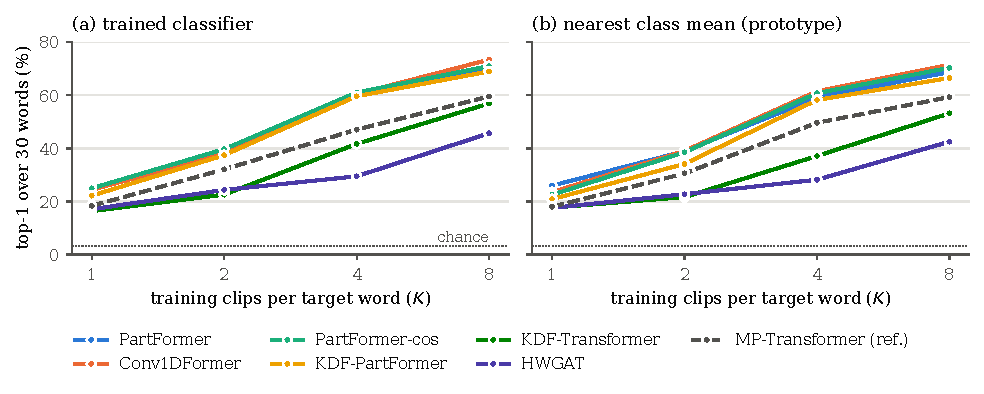
\includegraphics[width=\linewidth]{figures/uniform.pdf}
\caption{Uniform protocol (every word has $K$ clips): top-1 over 30 words. (a) Trained
classifier. (b) Nearest class mean of the same embeddings. The dotted line is chance
(3.3\,\%).}
\label{fig:uniform}
\end{figure}

\begin{table}[t]
\centering
\small
\caption{Uniform protocol: top-1 accuracy (\%) over 30 words when every word has $K$ training clips (same 240 test clips as the scarce protocol). Chance is 3.3\,\%.}
\label{tab:uniform}
\begin{tabular}{lcccc}
\toprule
Model & $K=1$ & $K=2$ & $K=4$ & $K=8$ \\
\midrule
MP-Transformer & 18.3\,{\scriptsize$\pm$4.0} & 32.1\,{\scriptsize$\pm$2.6} & 47.1\,{\scriptsize$\pm$2.9} & 59.5\,{\scriptsize$\pm$3.2} \\
\midrule
HWGAT & 17.1\,{\scriptsize$\pm$3.8} & 24.4\,{\scriptsize$\pm$5.1} & 29.5\,{\scriptsize$\pm$4.9} & 45.7\,{\scriptsize$\pm$6.0} \\
\midrule
KDF-Transformer & 16.4\,{\scriptsize$\pm$9.0} & 22.6\,{\scriptsize$\pm$2.2} & 41.7\,{\scriptsize$\pm$1.1} & 56.9\,{\scriptsize$\pm$4.4} \\
\quad $-$both (mixup+LS only) & 18.5\,{\scriptsize$\pm$5.4} & 28.0\,{\scriptsize$\pm$4.2} & 46.2\,{\scriptsize$\pm$5.5} & 55.9\,{\scriptsize$\pm$5.6} \\
\midrule
PartFormer & 24.9\,{\scriptsize$\pm$4.8} & 39.1\,{\scriptsize$\pm$2.7} & 60.2\,{\scriptsize$\pm$1.6} & 69.9\,{\scriptsize$\pm$4.3} \\
PartFormer-cos & \textbf{25.0\,{\scriptsize$\pm$4.3}} & \textbf{39.7\,{\scriptsize$\pm$4.5}} & \textbf{61.0\,{\scriptsize$\pm$2.6}} & 71.0\,{\scriptsize$\pm$6.6} \\
Conv1DFormer & 24.4\,{\scriptsize$\pm$5.8} & 38.2\,{\scriptsize$\pm$5.5} & 60.5\,{\scriptsize$\pm$4.3} & \textbf{73.4\,{\scriptsize$\pm$7.2}} \\
KDF-PartFormer & 22.2\,{\scriptsize$\pm$4.6} & 37.4\,{\scriptsize$\pm$3.0} & 59.6\,{\scriptsize$\pm$0.8} & 69.0\,{\scriptsize$\pm$4.5} \\
\bottomrule
\end{tabular}
\end{table}


When every word has $K$ clips (\cref{fig:uniform}a, \cref{tab:uniform}), the ranking is the
same. The part models reach 22--25\,\% top-1 over 30 words at $K{=}1$ (MP-Transformer
\MPuniA\,\%) and 69--73\,\% at $K{=}8$ (MP-Transformer \MPuniD\,\%). The spread among the four
part models is within one seed standard deviation at every $K$.

\subsection{What does not help}

\begin{table}[t]
\centering
\small
\caption{Koopman/DMD ablation on the scarce protocol: target-word top-1 (\%). DMD: Hankel-DMD spectrum and mode branch; KH: class-wise Koopman head. The first five rows share the landmark Transformer backbone.}
\label{tab:kdf}
\footnotesize
\setlength{\tabcolsep}{4pt}
\begin{tabular}{l>{\raggedright\arraybackslash}p{2.9cm}cccc}
\toprule
Model & Components & $K=1$ & $K=2$ & $K=4$ & $K=8$ \\
\midrule
MP-Transformer & -- & 6.2\,{\scriptsize$\pm$3.0} & 23.5\,{\scriptsize$\pm$7.5} & 44.7\,{\scriptsize$\pm$11.7} & 52.8\,{\scriptsize$\pm$11.7} \\
MP-Transformer + mixup/LS & mixup+LS & 4.3\,{\scriptsize$\pm$2.6} & 17.3\,{\scriptsize$\pm$10.1} & 36.6\,{\scriptsize$\pm$7.7} & 46.5\,{\scriptsize$\pm$10.6} \\
KDF $-$Koopman head & mixup+LS, DMD & 6.3\,{\scriptsize$\pm$4.8} & 18.1\,{\scriptsize$\pm$13.8} & 36.2\,{\scriptsize$\pm$16.4} & 50.2\,{\scriptsize$\pm$11.4} \\
KDF $-$DMD & mixup+LS, KH & 6.4\,{\scriptsize$\pm$1.9} & 13.0\,{\scriptsize$\pm$11.9} & 39.8\,{\scriptsize$\pm$15.7} & 54.3\,{\scriptsize$\pm$10.2} \\
KDF-Transformer & mixup+LS, DMD, KH & 7.5\,{\scriptsize$\pm$1.2} & 22.1\,{\scriptsize$\pm$11.7} & 37.7\,{\scriptsize$\pm$12.7} & 54.1\,{\scriptsize$\pm$9.6} \\
\midrule
PartFormer & part front end, mixup+LS & 17.0\,{\scriptsize$\pm$3.5} & 37.2\,{\scriptsize$\pm$10.2} & 54.7\,{\scriptsize$\pm$7.1} & 70.4\,{\scriptsize$\pm$10.8} \\
KDF-PartFormer & part front end, mixup+LS, DMD, KH & 9.8\,{\scriptsize$\pm$3.2} & 36.6\,{\scriptsize$\pm$6.9} & 55.6\,{\scriptsize$\pm$9.5} & 64.2\,{\scriptsize$\pm$9.6} \\
\bottomrule
\end{tabular}
\end{table}


\paragraph{Koopman/DMD features.}
\Cref{tab:kdf} shows that none of the KDF components produces a reliable gain on the landmark
backbone. KDF-Transformer is within 2.3 points of MP-Transformer at $K\in\{1,2,8\}$, with no
significant difference, and 7 points worse at $K{=}4$. Its ablations fall within the seed
spread of the full model. On the part backbone, adding the DMD branch and the Koopman head
(KDF-PartFormer) \emph{lowers} target accuracy at $K{=}1$ (\KPFtgtA\ vs.\ \PFtgtA) and $K{=}8$
(\KPFtgtD\ vs.\ \PFtgtD). With 30 frames per clip and $d{=}8$ delays, the Hankel matrices are
short, and a few noisy eigenvalues appear to add variance rather than information.

\paragraph{Mixup and label smoothing.}
Applied to MP-Transformer alone, mixup and label smoothing reduce target accuracy at every
$K$ in the scarce protocol. The drop is significant at $K\in\{2,4,8\}$ (6--8 points,
\cref{tab:paired}). The part models' gains are therefore not due to these regularisers:
they come despite them.

\paragraph{Cosine classifier.}
PartFormer-cos is below PartFormer at $K{=}1$ (\PFCtgtA\ vs.\ \PFtgtA) and slightly above it
at $K\in\{2,4\}$. None of these differences is large compared with the seed spread, and the
cosine head does not reduce absorption at $K{=}1$ (\PFCabsA\ vs.\ \PFabsA\,\%).

\begin{table}[t]
\centering
\small
\caption{Trained linear head versus a nearest-class-mean (prototype) classifier built from the same embeddings of the training clips, uniform protocol, top-1 (\%) over 30 words.}
\label{tab:proto}
\begin{tabular}{lcccccccc}
\toprule
 & \multicolumn{2}{c}{$K=1$} & \multicolumn{2}{c}{$K=2$} & \multicolumn{2}{c}{$K=4$} & \multicolumn{2}{c}{$K=8$} \\
\cmidrule(lr){2-3}\cmidrule(lr){4-5}\cmidrule(lr){6-7}\cmidrule(lr){8-9}
Model & head & proto & head & proto & head & proto & head & proto \\
\midrule
MP-Transformer & 18.3 & 18.0 & 32.1 & 30.6 & 47.1 & \textbf{49.6} & 59.5 & 59.3 \\
HWGAT & 17.1 & \textbf{17.6} & 24.4 & 22.7 & 29.5 & 28.2 & 45.7 & 42.5 \\
KDF-Transformer & 16.4 & \textbf{17.7} & 22.6 & 21.7 & 41.7 & 37.1 & 56.9 & 53.2 \\
MP-Transformer + mixup/LS & 18.5 & 17.6 & 28.0 & 25.7 & 46.2 & \textbf{46.4} & 55.9 & \textbf{56.4} \\
PartFormer & 24.9 & \textbf{25.9} & 39.1 & 38.9 & 60.2 & 59.1 & 69.9 & 68.7 \\
PartFormer-cos & 25.0 & 22.5 & 39.7 & 38.5 & 61.0 & 60.8 & 71.0 & 70.3 \\
Conv1DFormer & 24.4 & 23.5 & 38.2 & \textbf{39.0} & 60.5 & \textbf{61.5} & 73.4 & 71.4 \\
KDF-PartFormer & 22.2 & 20.9 & 37.4 & 34.1 & 59.6 & 58.2 & 69.0 & 66.5 \\
\bottomrule
\end{tabular}
\end{table}


\paragraph{Prototype versus trained head.}
If the linear head were the bottleneck at small $K$, a nearest-class-mean classifier on the
same embeddings should beat it~\citep{snell2017proto,chen2019closer}. \Cref{tab:proto} and
\cref{fig:uniform}b show that the two stay within 5 points of each other for every
model and budget, and the head is ahead in 24 of 32 cells. At $K\le8$ the quality of the
embedding, not the classifier on top of it, sets the accuracy.

\paragraph{Graph attention and spectral inputs.}
HWGAT, the only graph model we report, is the weakest or second-weakest model at every budget in every protocol. For example,
on the scarce protocol its overall accuracy is 17 points below MP-Transformer at $K{=}1$
($p<10^{-19}$). A linear probe on simple temporal statistics of its 27-joint skeleton input
reaches 58.5\,\% on the rich words at $K{=}8$, compared with 52.4\,\% for the 225-dimensional
landmark input.\footnote{Logistic regression on the per-clip mean, standard deviation and velocity standard deviation of each coordinate; scarce $K{=}8$, 3 seeds. This probe is not part of \texttt{make\_tables.py}.} This points to the model or its training, not its input, as the limitation.
HWGAT was designed for a corpus with far more data per word~\citep{patra2024hwgat} and may
need a different recipe. CWT-Transformer is competitive on the target words at $K{=}8$
(+9.1 points over MP-Transformer, $p{=}0.005$) but not overall.

% ==========================================================================================
\section{Discussion}

Taken together, the results give a consistent picture of ISLR with 1--8 examples per word.
What helps is the right \emph{structure} in the input encoder. This means treating hands,
body and face as separate parts, sharing the hand encoder across both hands, keeping hand
position and handshape as separate views, and modelling missing detections explicitly. These
choices add no parameters (PartFormer has 0.40\,M parameters, MP-Transformer 0.43\,M) and help
at every budget and in both protocols. What does not help, in our experiments, is additional
machinery on top of a given encoder: dynamical features, cosine or prototype classifiers,
and stronger regularisation.

The scarce-in-rich results carry a practical warning. When a new word is added to an
existing recogniser with a few recordings, standard training makes the model assign most of
the new word's clips to old words. More data for the old words makes this worse, not better.
Evaluations that report only aggregate accuracy hide this: on our scarce protocol overall
top-1 rises by only 10--14 points from $K{=}1$ to $K{=}8$, while target-word accuracy rises
by 47--58 points (\cref{tab:scarce_all,tab:scarce}).

% ==========================================================================================
\section{Limitations}\label{sec:limits}

\begin{itemize}
  \item \textbf{Scale.} One corpus, 30 words and 634 clips. Each seed has 62 target test
  clips, so per-seed estimates are noisy. Our conclusions rest on paired tests over the pooled
  seeds (186 target clips), but effects smaller than about 5 points cannot be resolved.
  \item \textbf{Withheld baselines.} ST-GCN, CTR-GCN, TD-GCN and PGF-SLR were trained, but an
  audit found implementation errors (input normalisation over the wrong axes, and a lossy part
  pooling), so we do not report them. Corrected runs are in progress, and the tables will be
  regenerated with the same script.
  \item \textbf{Confounds in the part models.} Besides factorising the input, the part models
  see the lips (MP-Transformer does not). The MP-Transformer + mixup/LS control rules out the
  regularisers, but we have not yet ablated the lip token or the individual design choices of
  the front end.
  \item \textbf{One recipe.} All models share one set of hyper-parameters and a fixed step
  budget. This is fair by construction but may disadvantage models that need a different
  learning rate or longer training (HWGAT in particular).
  \item \textbf{Identities.} INCLUDE sessions are inferred from camera counters, and ISL500
  sessions are assumed to be single signers. Errors in either could leak a signer between
  train and test.
  \item \textbf{Landmarks only.} We do not use RGB input, pre-training or cross-lingual
  transfer~\citep{selvaraj2022openhands}. Our pipeline supports pre-training, but it was not
  part of this study.
\end{itemize}

\paragraph{Ethics and data.}
All sources are public research corpora, used under their licences. CISLR is gated and is
used under its terms. We redistribute landmarks and predictions only where the source licence
allows. No Deaf signers were involved in designing this study. Any deployment of low-data
recognisers should involve the Deaf community and should not be treated as a substitute for
interpreters.

% ==========================================================================================
\section{Conclusion}

Under a controlled low-data protocol for isolated ISL recognition, a part-factorised
landmark encoder improves accuracy on words with 1--8 training clips by 11--17 points over a
landmark Transformer of the same size. Dynamical features, cosine or prototype classifiers
and extra regularisation give no reliable gain. Rare words embedded in a larger vocabulary
are mostly absorbed by common words, and more data for the common words makes this worse. We
hope the protocol and released predictions make future low-data SLR results easier to
compare.

\paragraph{Reproducibility.}
Every number in this paper is produced from the per-run outputs by
\texttt{paper/make\_tables.py}. The runs themselves are produced by
\texttt{lowdata.py sweep} with the grids \texttt{isl40\_scarce}, \texttt{isl40\_uniform} and \texttt{isl40\_vocab} in \texttt{islr/lowdata/configs/}
(\cref{app:repro}).

\bibliographystyle{plainnat}
\bibliography{refs}

% ==========================================================================================
\clearpage
\appendix
\section{Additional results}

\begin{table}[t]
\centering
\small
\caption{Scarce protocol: top-1 accuracy (\%) on the 22 rich words (178 test clips per seed). Their training data are the same for every $K$; only the target words change.}
\label{tab:rich}
\begin{tabular}{lcccc}
\toprule
Model & $K=1$ & $K=2$ & $K=4$ & $K=8$ \\
\midrule
MP-BiLSTM & 63.6\,{\scriptsize$\pm$2.6} & 61.6\,{\scriptsize$\pm$3.4} & 60.3\,{\scriptsize$\pm$3.2} & 61.0\,{\scriptsize$\pm$2.4} \\
MP-Transformer & 68.8\,{\scriptsize$\pm$2.4} & 67.6\,{\scriptsize$\pm$2.3} & 66.9\,{\scriptsize$\pm$3.3} & 65.9\,{\scriptsize$\pm$4.3} \\
\midrule
HWGAT & 47.4\,{\scriptsize$\pm$3.1} & 48.8\,{\scriptsize$\pm$4.6} & 48.2\,{\scriptsize$\pm$5.0} & 49.9\,{\scriptsize$\pm$2.5} \\
\midrule
FFT-BiLSTM & 60.4\,{\scriptsize$\pm$3.5} & 61.8\,{\scriptsize$\pm$4.8} & 59.5\,{\scriptsize$\pm$1.0} & 61.2\,{\scriptsize$\pm$2.5} \\
CWT-BiLSTM & 62.0\,{\scriptsize$\pm$4.2} & 59.3\,{\scriptsize$\pm$4.1} & 57.2\,{\scriptsize$\pm$1.8} & 58.9\,{\scriptsize$\pm$2.5} \\
CWT-Transformer & 66.8\,{\scriptsize$\pm$2.6} & 68.7\,{\scriptsize$\pm$1.4} & 65.4\,{\scriptsize$\pm$3.1} & 65.7\,{\scriptsize$\pm$3.6} \\
\midrule
KDF-Transformer & 67.9\,{\scriptsize$\pm$5.0} & 66.4\,{\scriptsize$\pm$2.5} & 65.8\,{\scriptsize$\pm$5.4} & 62.6\,{\scriptsize$\pm$6.1} \\
\quad $-$DMD & 65.3\,{\scriptsize$\pm$2.7} & 65.6\,{\scriptsize$\pm$2.6} & 66.3\,{\scriptsize$\pm$3.6} & 64.4\,{\scriptsize$\pm$2.7} \\
\quad $-$Koopman head & 66.0\,{\scriptsize$\pm$2.3} & 65.4\,{\scriptsize$\pm$3.3} & 64.9\,{\scriptsize$\pm$4.2} & 63.1\,{\scriptsize$\pm$7.5} \\
\quad $-$both (mixup+LS only) & 68.1\,{\scriptsize$\pm$1.0} & 66.2\,{\scriptsize$\pm$4.7} & 65.4\,{\scriptsize$\pm$4.1} & 65.1\,{\scriptsize$\pm$7.2} \\
\midrule
PartFormer & \textbf{81.9\,{\scriptsize$\pm$6.2}} & 80.2\,{\scriptsize$\pm$3.9} & 79.9\,{\scriptsize$\pm$3.0} & 79.4\,{\scriptsize$\pm$1.6} \\
PartFormer-cos & 80.6\,{\scriptsize$\pm$2.8} & \textbf{81.8\,{\scriptsize$\pm$3.7}} & 79.6\,{\scriptsize$\pm$4.1} & 79.0\,{\scriptsize$\pm$2.0} \\
Conv1DFormer & 81.4\,{\scriptsize$\pm$4.0} & 81.8\,{\scriptsize$\pm$4.0} & \textbf{80.8\,{\scriptsize$\pm$3.3}} & \textbf{80.4\,{\scriptsize$\pm$4.0}} \\
KDF-PartFormer & 79.9\,{\scriptsize$\pm$3.8} & 77.2\,{\scriptsize$\pm$1.3} & 77.9\,{\scriptsize$\pm$3.3} & 76.6\,{\scriptsize$\pm$2.7} \\
\bottomrule
\end{tabular}
\end{table}

\begin{table}[t]
\centering
\small
\caption{Absorption: percentage of target-word test clips predicted as one of the 22 rich words (lower is better; best in bold).}
\label{tab:absorb}
\begin{tabular}{lcccc}
\toprule
Model & $K=1$ & $K=2$ & $K=4$ & $K=8$ \\
\midrule
MP-BiLSTM & 93.0\,{\scriptsize$\pm$1.6} & 71.0\,{\scriptsize$\pm$13.5} & 53.6\,{\scriptsize$\pm$8.5} & 39.7\,{\scriptsize$\pm$11.9} \\
MP-Transformer & 91.4\,{\scriptsize$\pm$1.2} & 72.9\,{\scriptsize$\pm$10.8} & 51.2\,{\scriptsize$\pm$14.6} & 44.0\,{\scriptsize$\pm$12.4} \\
\midrule
HWGAT & 98.4\,{\scriptsize$\pm$1.6} & 88.0\,{\scriptsize$\pm$4.7} & 78.2\,{\scriptsize$\pm$5.0} & 61.9\,{\scriptsize$\pm$6.0} \\
\midrule
FFT-BiLSTM & 89.7\,{\scriptsize$\pm$3.9} & 70.5\,{\scriptsize$\pm$1.0} & 61.1\,{\scriptsize$\pm$5.6} & 45.7\,{\scriptsize$\pm$8.6} \\
CWT-BiLSTM & 88.3\,{\scriptsize$\pm$4.0} & 68.7\,{\scriptsize$\pm$9.6} & 52.9\,{\scriptsize$\pm$13.3} & 46.7\,{\scriptsize$\pm$14.2} \\
CWT-Transformer & 90.5\,{\scriptsize$\pm$3.3} & 69.0\,{\scriptsize$\pm$9.6} & 53.1\,{\scriptsize$\pm$13.7} & 34.6\,{\scriptsize$\pm$16.4} \\
\midrule
KDF-Transformer & 91.0\,{\scriptsize$\pm$1.0} & 73.5\,{\scriptsize$\pm$11.7} & 56.5\,{\scriptsize$\pm$10.6} & 40.4\,{\scriptsize$\pm$4.8} \\
\quad $-$DMD & 92.7\,{\scriptsize$\pm$0.7} & 82.8\,{\scriptsize$\pm$13.9} & 54.9\,{\scriptsize$\pm$16.5} & 44.2\,{\scriptsize$\pm$10.8} \\
\quad $-$Koopman head & 92.7\,{\scriptsize$\pm$3.5} & 80.9\,{\scriptsize$\pm$12.9} & 60.3\,{\scriptsize$\pm$17.9} & 40.1\,{\scriptsize$\pm$7.2} \\
\quad $-$both (mixup+LS only) & 95.7\,{\scriptsize$\pm$2.6} & 80.2\,{\scriptsize$\pm$11.8} & 59.5\,{\scriptsize$\pm$9.2} & 50.2\,{\scriptsize$\pm$11.3} \\
\midrule
PartFormer & \textbf{78.4\,{\scriptsize$\pm$5.2}} & 61.8\,{\scriptsize$\pm$9.3} & 44.8\,{\scriptsize$\pm$7.9} & 28.5\,{\scriptsize$\pm$8.9} \\
PartFormer-cos & 84.5\,{\scriptsize$\pm$7.7} & \textbf{59.4\,{\scriptsize$\pm$6.8}} & 40.2\,{\scriptsize$\pm$4.3} & 29.4\,{\scriptsize$\pm$3.9} \\
Conv1DFormer & 83.6\,{\scriptsize$\pm$1.2} & 59.6\,{\scriptsize$\pm$13.2} & \textbf{39.0\,{\scriptsize$\pm$7.8}} & \textbf{27.0\,{\scriptsize$\pm$12.3}} \\
KDF-PartFormer & 88.1\,{\scriptsize$\pm$4.5} & 61.9\,{\scriptsize$\pm$5.5} & 43.4\,{\scriptsize$\pm$7.8} & 32.3\,{\scriptsize$\pm$10.0} \\
\bottomrule
\end{tabular}
\end{table}

\begin{table}[t]
\centering
\small
\caption{Scarce protocol: overall top-1 accuracy (\%) over all 30 words (240 test clips per seed).}
\label{tab:scarce_all}
\begin{tabular}{lcccc}
\toprule
Model & $K=1$ & $K=2$ & $K=4$ & $K=8$ \\
\midrule
MP-BiLSTM & 49.1\,{\scriptsize$\pm$2.6} & 52.2\,{\scriptsize$\pm$5.3} & 54.6\,{\scriptsize$\pm$4.0} & 58.7\,{\scriptsize$\pm$3.5} \\
MP-Transformer & 53.0\,{\scriptsize$\pm$2.3} & 56.4\,{\scriptsize$\pm$4.0} & 61.2\,{\scriptsize$\pm$5.6} & 62.6\,{\scriptsize$\pm$4.5} \\
\midrule
HWGAT & 35.7\,{\scriptsize$\pm$2.4} & 39.3\,{\scriptsize$\pm$4.2} & 40.7\,{\scriptsize$\pm$3.3} & 45.5\,{\scriptsize$\pm$4.1} \\
\midrule
FFT-BiLSTM & 47.3\,{\scriptsize$\pm$2.8} & 51.6\,{\scriptsize$\pm$2.9} & 53.3\,{\scriptsize$\pm$2.6} & 57.4\,{\scriptsize$\pm$3.3} \\
CWT-BiLSTM & 49.1\,{\scriptsize$\pm$3.0} & 51.1\,{\scriptsize$\pm$1.5} & 53.2\,{\scriptsize$\pm$3.9} & 56.6\,{\scriptsize$\pm$2.6} \\
CWT-Transformer & 52.2\,{\scriptsize$\pm$3.0} & 58.8\,{\scriptsize$\pm$2.3} & 60.3\,{\scriptsize$\pm$3.8} & 64.8\,{\scriptsize$\pm$3.2} \\
\midrule
KDF-Transformer & 52.6\,{\scriptsize$\pm$4.6} & 55.1\,{\scriptsize$\pm$4.7} & 58.6\,{\scriptsize$\pm$7.0} & 60.4\,{\scriptsize$\pm$7.0} \\
\quad $-$DMD & 50.4\,{\scriptsize$\pm$1.8} & 52.2\,{\scriptsize$\pm$4.2} & 59.5\,{\scriptsize$\pm$6.9} & 61.9\,{\scriptsize$\pm$4.6} \\
\quad $-$Koopman head & 50.9\,{\scriptsize$\pm$3.1} & 53.4\,{\scriptsize$\pm$6.2} & 57.6\,{\scriptsize$\pm$7.5} & 59.9\,{\scriptsize$\pm$8.5} \\
\quad $-$both (mixup+LS only) & 51.9\,{\scriptsize$\pm$1.8} & 53.7\,{\scriptsize$\pm$4.8} & 58.1\,{\scriptsize$\pm$5.3} & 60.5\,{\scriptsize$\pm$7.3} \\
\midrule
PartFormer & \textbf{65.6\,{\scriptsize$\pm$5.1}} & 69.3\,{\scriptsize$\pm$5.4} & 73.5\,{\scriptsize$\pm$3.9} & 77.1\,{\scriptsize$\pm$3.6} \\
PartFormer-cos & 63.2\,{\scriptsize$\pm$2.1} & \textbf{71.0\,{\scriptsize$\pm$4.5}} & 74.3\,{\scriptsize$\pm$4.2} & 76.7\,{\scriptsize$\pm$2.5} \\
Conv1DFormer & 64.3\,{\scriptsize$\pm$3.2} & 71.0\,{\scriptsize$\pm$6.6} & \textbf{75.7\,{\scriptsize$\pm$4.6}} & \textbf{78.1\,{\scriptsize$\pm$5.6}} \\
KDF-PartFormer & 62.2\,{\scriptsize$\pm$3.2} & 66.9\,{\scriptsize$\pm$2.7} & 72.3\,{\scriptsize$\pm$4.6} & 73.4\,{\scriptsize$\pm$4.5} \\
\bottomrule
\end{tabular}
\end{table}

\begin{table}[t]
\centering
\small
\caption{Uniform protocol: top-5 accuracy (\%).}
\label{tab:uniform5}
\begin{tabular}{lcccc}
\toprule
Model & $K=1$ & $K=2$ & $K=4$ & $K=8$ \\
\midrule
MP-Transformer & 49.4\,{\scriptsize$\pm$3.1} & 60.9\,{\scriptsize$\pm$7.6} & 80.4\,{\scriptsize$\pm$4.3} & 85.0\,{\scriptsize$\pm$4.0} \\
\midrule
HWGAT & 49.5\,{\scriptsize$\pm$3.6} & 55.4\,{\scriptsize$\pm$5.4} & 68.8\,{\scriptsize$\pm$4.1} & 79.2\,{\scriptsize$\pm$3.0} \\
\midrule
KDF-Transformer & 41.4\,{\scriptsize$\pm$7.7} & 58.3\,{\scriptsize$\pm$8.6} & 71.7\,{\scriptsize$\pm$1.3} & 85.0\,{\scriptsize$\pm$6.4} \\
\quad $-$both (mixup+LS only) & 46.9\,{\scriptsize$\pm$6.9} & 62.8\,{\scriptsize$\pm$5.4} & 78.4\,{\scriptsize$\pm$6.2} & 85.1\,{\scriptsize$\pm$6.5} \\
\midrule
PartFormer & 55.7\,{\scriptsize$\pm$6.9} & 73.1\,{\scriptsize$\pm$6.5} & 87.1\,{\scriptsize$\pm$5.3} & \textbf{91.1\,{\scriptsize$\pm$5.0}} \\
PartFormer-cos & \textbf{57.6\,{\scriptsize$\pm$8.5}} & \textbf{73.9\,{\scriptsize$\pm$5.7}} & 86.4\,{\scriptsize$\pm$5.5} & 89.2\,{\scriptsize$\pm$5.3} \\
Conv1DFormer & 55.1\,{\scriptsize$\pm$7.2} & 72.8\,{\scriptsize$\pm$8.7} & \textbf{87.4\,{\scriptsize$\pm$2.3}} & 90.1\,{\scriptsize$\pm$5.9} \\
KDF-PartFormer & 53.5\,{\scriptsize$\pm$9.9} & 71.2\,{\scriptsize$\pm$7.3} & 87.1\,{\scriptsize$\pm$3.4} & 88.9\,{\scriptsize$\pm$6.2} \\
\bottomrule
\end{tabular}
\end{table}

\begin{table}[t]
\centering
\small
\caption{Per-word top-1 (\%) on the 8 target words, scarce protocol, mean over 3 seeds.}
\label{tab:perword}
\begin{tabular}{lcccc}
\toprule
 & \multicolumn{2}{c}{MP-Transformer} & \multicolumn{2}{c}{PartFormer} \\
\cmidrule(lr){2-3}\cmidrule(lr){4-5}
Word & $K=1$ & $K=8$ & $K=1$ & $K=8$ \\
\midrule
eat & 0 & 8 & 0 & 33 \\
go & 10 & 77 & 5 & 86 \\
hello & 7 & 75 & 26 & 77 \\
help & 14 & 65 & 32 & 74 \\
no & 4 & 42 & 12 & 80 \\
please & 6 & 40 & 11 & 79 \\
water & 0 & 37 & 17 & 64 \\
yes & 5 & 37 & 18 & 61 \\
\bottomrule
\end{tabular}
\end{table}


\Cref{tab:perword} breaks the target accuracy down by word. \emph{Eat} is the hardest word
for both models: PartFormer recognises 33\,\% of its test clips at $K{=}8$, and MP-Transformer
8\,\%. The largest gains of the part model are on \emph{no} and \emph{please} (about 38 points each at $K{=}8$).

\FloatBarrier
\section{Reproducing the results}\label{app:repro}

\begin{verbatim}
pip install -r requirements.txt
export STORES=/path/to/stores      # landmark stores built by `lowdata.py data`
for g in isl40_scarce isl40_uniform isl40_vocab; do
  python lowdata.py sweep --out sweeps \
      --grid islr/lowdata/configs/$g.json
done
python lowdata.py report --out sweeps
# add --include-graph once the graph rerun is done
python paper/make_tables.py --sweeps sweeps
cd paper && latexmk -pdf main.tex
\end{verbatim}

A single run is
\begin{verbatim}
python lowdata.py run --stores S --model partformer \
    --protocol scarce --shots 4 --seed 0
\end{verbatim}
Each run directory contains \texttt{result.json} (metrics and configuration),
\texttt{split.json} (the exact train and test clip keys) and \texttt{preds.npz} (per-clip
predictions and logits). The paired tests use the latter two.

\end{document}
